\documentclass[14pt]{beamer}

\title[SUE]{Safe User Expirience Plugin}
\subtitle{june-july 2020 Project}
\author[Team 36]{Syeda Reeha Quasar, Kahkasha Parveen, Mahi Monga}
\date{June 2020}

\usepackage{graphicx}
\graphicspath{ {./images/}}

\usetheme{Warsaw}

\begin{document}

\begin{frame}
    \titlepage
\end{frame}

\begin{frame}
    \frametitle{Overview}
    Our Project aims to provide an extension \ plugin which woul protect the users from phishing sites or sites containing malware which could cause harm to the user if user visits certain sites.
    Our aim is to built a solution in cybersecurity domain which is the need for the current time and provide users a safe and secure surfing experience.
\end{frame}

\begin{frame}
    \frametitle{Technologies Used:}
    \begin{enumerate}
        \item{Python}
        \item{HTML}
        \item{CSS}
        \item{JavaScript}
    \end{enumerate}
\end{frame}

\begin{frame}
    \frametitle{Description}
    We are going to build and train an ML model which would detect the sites which can be steal your data or personal information and cause harm to your device.
    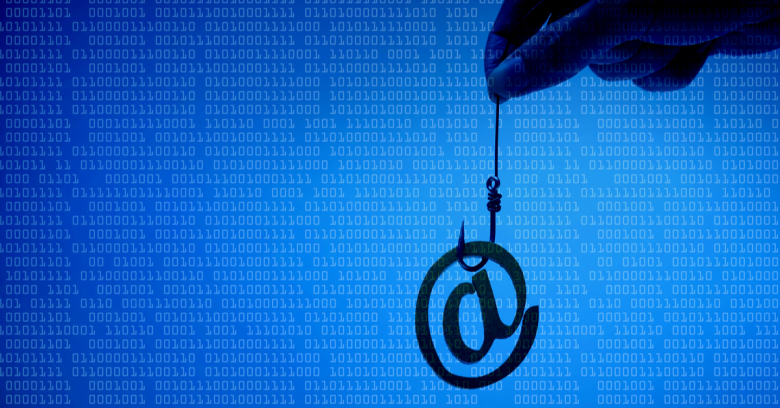
\includegraphics{shutterstock_593626601}
    \href{https://developer.chrome.com/extensions/getstarted}{\beamergobutton{How to make Extension}}
\end{frame}

\begin{frame}
    \frametitle{Work Flow}
    \begin{enumerate}
        \item{Data extraction / collection}
        \item{Data manipulation}
        \item{Data summarization}
        \item{Loading data and dataset}
        \item{Data visualisation}
        \item{Writing algorithm}
        \item{Build models}
        \item{Selecting best model}
        \item{Test and make predictions}
        \item{Making extension}
        \item{Loading our model into extension}
        \item{Try and deploy it…}
    \end{enumerate}
\end{frame}

\begin{frame}
    \frametitle{references}
    \href{https://github.com/arvind-rs/phishing_detector}{\beamergobutton{git repo 1}}
    \href{https://github.com/faizann24/phishytics-machine-learning-for-phishing}{\beamergobutton{git repo 2}}
    \href{https://machinelearningmastery.com/machine-learning-in-python-step-by-step/}{\beamergobutton{ML model building}}
\end{frame}


\end{document}
